\section{MDL Beyond a Single Shard is Hard}
\label{sec:mdl:zookeeper}

\todo{Change to 'do existing systems provide \mdl{}. Say we have a new consistency model. Do existing provide it? Surprisingly it appears single-shard implementations do not, though there is a design for it on a single shard. Then structure single-shard \mdl{} and multi-shard \mdl{}.}

\begin{figure}[!tb]
    \centering
    % 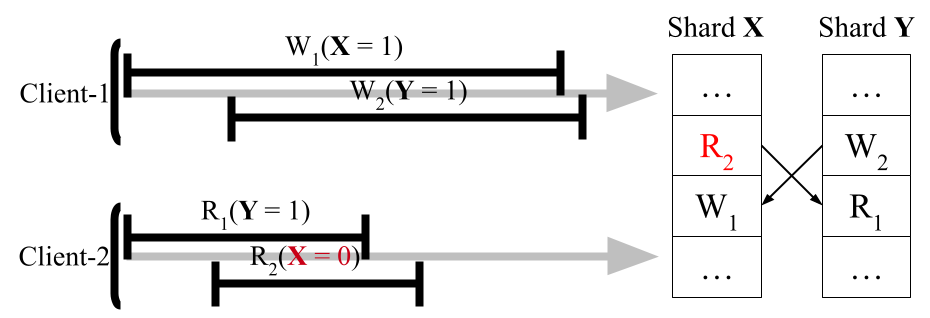
\includegraphics[width=\linewidth]{figs/somet.png}
    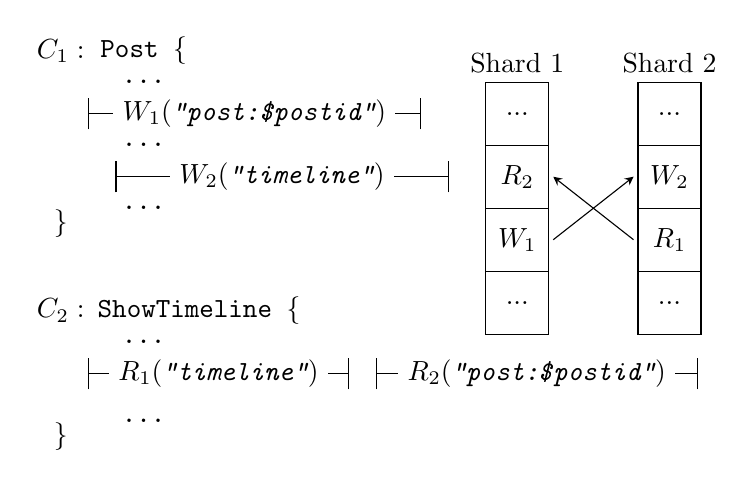
\begin{tikzpicture}

% Shard X
\node (shardy) [
    xshift=-\textwidth+125,
    align=center,
    anchor=south,
    yshift=0.4cm,
    fill=none
] {Shard 1};
\node (appbox) [draw,
    minimum size=0.8cm,
    xshift=-\textwidth+125,
    align=center,
    yshift=0cm
] {...};

\node (linstore) [draw,
    minimum size=0.8cm,
    align=center,
    xshift=-\textwidth+125,
    yshift=-0.8cm
] {$R_2$};

\node (appbox) [draw,
    minimum size=0.8cm,
    xshift=-\textwidth+125,
    align=center,
    yshift=-1.6cm
] {$W_1$};

\node (linstore) [draw,
    minimum size=0.8cm,
    align=center,
    xshift=-\textwidth+125,
    yshift=-2.4cm
] {...};


% Shard Y
\node (shardy) [
    xshift=-\textwidth+180,
    align=center,
    anchor=south,
    yshift=0.4cm,
    fill=none
] {Shard 2};

\node (mdapp) [draw,
    minimum size=0.8cm,
    xshift=-\textwidth+180,
    align=center,
    yshift=0cm
] {...};

\node (mdlinstore) [draw,
    minimum size=0.8cm,
    xshift=-\textwidth+180,
    align=center,
    yshift=-0.8cm
] {$W_2$};

\node (appbox) [draw,
    minimum size=0.8cm,
    xshift=-\textwidth+180,
    align=center,
    yshift=-1.6cm
] {$R_1$};

\node (linstore) [draw,
    minimum size=0.8cm,
    align=center,
    xshift=-\textwidth+180,
    yshift=-2.4cm
] {...};

\draw [stealth-](-\textwidth+138, -0.8) --  node[midway,fill=none]{}(-\textwidth+167,-1.6);


\draw [stealth-](-\textwidth+167,-0.8) --  node[midway,fill=none,align=center]{}(-\textwidth+138, -1.6);

%-------------------------------------
%-------------------------------------
\node (c1) [
    minimum size=0.2cm,
    xshift=-\textwidth-40,
    align=center,
    yshift=0.8cm,
    fill=none
] {$C_1:$};
\node (post1) [
    xshift=-\textwidth-10,
    align=center,
    yshift=0.8cm,
    fill=none
] {\texttt{Post \{}};
\node (post2) [
    xshift=-\textwidth-10,
    align=center,
    yshift=0.4cm,
    fill=none
] {\texttt{...}};
\node (post3) [
    xshift=-\textwidth-10,
    align=center,
    yshift=-0.4cm,
    fill=none
] {\texttt{...}};
\node (post4) [
    xshift=-\textwidth-10,
    align=center,
    yshift=-1.2cm,
    fill=none
] {\texttt{...}};
\node (post5) [
    xshift=-\textwidth-40,
    align=center,
    yshift=-1.4cm,
    fill=none
] {\texttt{\}}};

%------------------------------
\node (c2) [
    minimum size=0.2cm,
    xshift=-\textwidth-40,
    align=center,
    yshift=-2.5cm,
    fill=none
] {$C_2:$};

\node (timeline1) [
    xshift=-\textwidth+10,
    align=center,
    yshift=-2.5cm,
    fill=none
] {\texttt{ShowTimeline \{}};
\node (timeline2) [
    xshift=-\textwidth-10,
    align=center,
    yshift=-2.9cm,
    fill=none
] {\texttt{...}};
\node (timeline3) [
    xshift=-\textwidth-10,
    align=center,
    yshift=-3.9cm,
    fill=none
] {\texttt{...}};
\node (timelin4) [
    xshift=-\textwidth-40,
    align=center,
    yshift=-4.1cm,
    fill=none
] {\texttt{\}}};


% \node (c1) [
%     minimum size=0.2cm,
%     xshift=-\textwidth-40,
%     align=center,
%     yshift=0cm,
%     fill=none
% ] {$C_1:$};
% \node (post) [
%     xshift=-\textwidth-40,
%     align=center,
%     anchor=south,
%     yshift=0.4cm,
%     fill=none
% ] {\texttt{Post}};

% \node (c2) [
%     minimum size=0.2cm,
%     xshift=-\textwidth-40,
%     align=center,
%     yshift=-3.3cm,
%     fill=none
% ] {$C_2:$};

% \node (timeline) [
%     xshift=-\textwidth-20,
%     align=center,
%     anchor=south,
%     yshift=-2.9cm,
%     fill=none
% ] {\texttt{ShowTimeline}};

% W1
\draw [-](-\textwidth-30,0) --  node[midway,fill=white, align=center]{\textit{$W_1(\texttt{"post:\$postid"})$}}(-\textwidth+90, 0);
\draw [-](-\textwidth-30,-0-0.2) --  node[midway,fill=none, align=left, anchor=south]{}(-\textwidth-30,0+0.2);
\draw [-](-\textwidth+90, 0-0.2) --  node[midway,fill=none, align=left, anchor=south]{}(-\textwidth+90, 0+0.2);
% W2
\draw [-](-\textwidth-20,-0.8) --  node[midway,fill=white, align=center]{\textit{$W_2(\texttt{"timeline"})$}}(-\textwidth+100, -0.8);
\draw [-](-\textwidth-20,-0.8-0.2) --  node[midway,fill=none, align=left, anchor=south]{}(-\textwidth-20,-0.8+0.2);
\draw [-](-\textwidth+100, -0.8-0.2) --  node[midway,fill=none, align=left, anchor=south]{}(-\textwidth+100, -0.8+0.2);

% R1
\draw [-](-\textwidth-30,-3.3) --  node[midway,fill=white, align=center]{\textit{$R_1(\texttt{"timeline"})$}}(-\textwidth+64, -3.3);
\draw [-](-\textwidth-30,-3.3-0.2) --  node[midway,fill=none, align=left, anchor=south]{}(-\textwidth-30,-3.3+0.2);
\draw [-](-\textwidth+64, -3.3-0.2) --  node[midway,fill=none, align=left, anchor=south]{}(-\textwidth+64, -3.3+0.2);
% R2
\draw [-](-\textwidth+74,-3.3) --  node[midway,fill=white, align=center]{\textit{$R_2(\texttt{"post:\$postid"})$}}(-\textwidth+190, -3.3);
\draw [-](-\textwidth+74,-3.3-0.2) --  node[midway,fill=none, align=left, anchor=south]{}(-\textwidth+74,-3.3+0.2);
\draw [-](-\textwidth+190, -3.3-0.2) --  node[midway,fill=none, align=left, anchor=south]{}(-\textwidth+190, -3.3+0.2);

\end{tikzpicture}
    \caption{Example where two concurrent client processes each submit operations that touch shared keys. The first client issues concurrent operations from the Retwis \texttt{Post} function, while the second issues operations from the Retwis \texttt{ShowTimeline} function that have a real-time ordering guarantee between them. The keys \texttt{"post:\$postid"} and \texttt{"timeline"} are at different shards (1 and 2 respectively). Without coordination in the protocol, it is possible that $R_2$ arrives before $W_1$ at shard 1, and $W_2$ arrives before $R_1$ at shard 2. This would not provide a total order of operations and would result in $C_2$'s timeline showing a dangling posted object, violating the guarantees defined in \mdl{}.}
    \label{fig:concurrentbatches}
\end{figure}

Linearizability is a local property (or, composable), which means that every individual object in the system is linearizable if and only if the system as a whole is linearizable ~\cite{herlihy1990linearizability}. Locality makes constructing multi-sharded linearizable systems quite trivial: a multi-sharded system, where each shard is linearizable, is also linearizable as a whole.

\mdl{} is not a local property. 
% A system composed of two or more shards, where each individual \iocll{}, is not \iocll{} as a whole.
A system composed of two or more shards, where each individual \iocll{} shard orders operations independently, can lead to violations of \MDL{}'s total order guarantee, as demonstrated in figure ~\ref{fig:concurrentbatches}. 
This example comes directly from the Retwis codebase, where the \texttt{Post} and \texttt{ShowTimeline} functions are defined (the former is portrayed in full in figure ~\ref{fig:retwis-post2}). We next show how with the guarantees of IOC
Linearizability in a multi-sharded setting lost, the users of this application could see observe strange behavior.

Consider a common occurrence where \IOCL{} transformed versions of both \texttt{Post} and \texttt{ShowTimeline} are invoked concurrently by independent clients using the application, and the shared keys they touch reside at separate shards. Crucially, the concurrent operations issued by each function may arrive at their respective shards at any time. Finally, while there is a total order of operations that respects invocation order at each shard individually, there is no total order across the shards, or, in the system as a whole. Because of this, the second client sees a dangling object posted in a timeline, as described in section ~\ref{sec:motivation}.

% Two processes each issue two
% operations, one to key $X$ and the other to key $Y$, which reside on different
% shards. Process 1 writes $X$ then $Y$, and process 2 reads $Y$ then $X$. Suppose $W_2$ precedes $R_1$ at shard $Y$, causing it to return $Y=1$. Combined with
% process 2's issue-order, this implies $R_2$ must be serialized after $W_1$.
% But since operations can arrive at the shards in an arbitrary order, $R_2$ may
% precede $W_1$ and return $X=0$, violating \MDL{}.




Because \IOCL isn't local, constructing multi-sharded \iocll{} systems is hard.
There are several existing systems that could be used to provide
\multidispatch{} linearizability on a single shard. We briefly describe them and then show how they fail to extend to multiple shards.

\paragraph{Zookeeper.} To the best of our knowledge, Zookeeper~\cite{hunt2010zookeeper} is the
only existing work to account for (in its consistency model) an 
application process potentially issuing multiple operations concurrently. The authors denote it Asynchronous Linearizability
(or A-Linearizability)~\cite{hunt2010zookeeper}. But despite its name,
it differs from \MDL{} because Zookeeper allows
reads to return stale (i.e., non-linearizable) values. Besides providing weaker consistency guarantees than \mdl{}, Zookeeper also only provides those guarantees for a single-shard, assuming client data is small and can fit on a single machine in memory database.

\paragraph{Raft, etc.} To handle concurrent operations from the same process in the single shard setting, existing leader-based replicated-state-machine protocols (could) use
per-process sequence numbers~\cite{ongaro2014raft,lamport1998paxos,oki1988vr} to guarantee \MDL{} on one shard. Sequence numbers are assigned in the client 
library and increase monotonically. This provides sufficient information for
the leader to ensure each process's operations enter the log in an
order consistent with its issue order
(e.g., by queuing operations in sequence-number order).
\footnote{Zookeeper can be forced to
guarantee \MDL{} by issuing a \texttt{sync} operation before each read to prevent it from returning a stale value.}

\paragraph{Salus.} Salus is a block store that lets clients mount multiple volumes (similar to multiple shards) and preserves commit-order across operations. While this is akin to \mdl{} in multiple-shards, Salus only allows single writers per volume, thus eliminating cross client concurrency and trivially satisfying commit-order across multiple volumes.

\ak{I would delete this paragraph.} These protocols fail to 
guarantee \MDL{} across multiple shards for two reasons. First,
as mentioned, multiple shards
introduces the possibility for independent failures of operations. A first
operation at one shard may fail and need to be retried (e.g., due to
leader failure) while a second operation at another shard succeeds, and
its effects become visible to other processes. If both of these
operations were issued concurrently from the same process, 
this would violate \MDL{}'s suffix-closed failure semantics.

In the next section, we describe our new protocol, \sys{}, that tackles these
challenges and guarantees \multidispatch{} linearizability for a multi-shard
system.